% !TeX root = ../thesis.tex
% !TeX spellcheck = en_US

\section{Motivation}

	Traveling through a network of roads and paths often requires a computer system determining the optimal route from a source to a destination location.
	The software that solves this problem is often called a \emph{routing engine} and uses shortest path algorithms.
	A graph is used as the underlying data structure, which abstracts the real world into vertices and edges, representing roads and ways.
	Detailed information, such as surface conditions or the number of lanes, is usually added to the geometries of the graph via attributes, usually in form of key-value pairs.
	
	Algorithms for graph-based routing, such as Dijkstra or A*, are optimized and used in numerous scientific and real-world applications, including this work.
	To enhance performance in large networks, several speedup methods exist that further decrease query times allowing global routing requests to be answered within milliseconds.\footnote{Tested for a routing request from Hamburg, Germany to Beijing, China on \href{https://www.openstreetmap.org/directions?engine=fossgis\_osrm\_car&route=53.55\%2C10.00\%3B39.91\%2C116.39}{openstreetmap.org} using the OSRM car profile which is based on Contraction Hierarchies (s. \Cref{subsubsec:ch}). The HTTP request returned the result in under 215 ms -- including network latency of several milliseconds.}
	
	Aside from line-based shapes, which are very suitable for routing, the real world also consists of polygonal areas, which can not be abstracted to a single line, such as marketplaces, parking lots or parks.
	Classical routing algorithms can therefore only find routes along the outer edges of these polygons.
	To cross these open areas, auxiliary paths are added to connect opposite sides of polygons, which is a common practice in OpenStreetMap, a crowdsourced geospatial database.
	A few lines can be added by hand, but manually filling large areas or even a whole city with these auxiliary paths is not feasible.
	However, geometric routing algorithms exist that find so-called \term*[euclidean shortest path]{euclidean shortest paths} across open spaces in the presence of impassible obstacles, such as buildings or walls.
	There are two main strategies for geometric routing, which will both be covered in detail in \Cref{sec:geometric-routing}.
	
	A similar problem arises with the source and destination locations of real-world routing.
	These locations are often not part of roads or ways and therefore the underlying routing graph, which is the case for most addresses, \term*[point of interest]{points of interest} (\term[POI]{POIs}) or manually chosen locations.
	However, only objects in the routing graph are reachable by graph-based routing algorithms.
	Simple approaches to connect points to a graph (e.g. connecting to the nearest vertex) are often inaccurate.
	Such inaccuracies arise because the space between an arbitrary location and the road network may contain obstacles, such as walls or buildings.
	
	Even if only vertices of the routing graph are chosen, the quality of graph-based routing results is limited due to the abstractions of the road network.
	Missing sidewalks, inaccurate geometries and missing connections between parallel ways reduce the usefulness of graph-based routes, especially for routes determined for pedestrians.
	
	\section{Problem and contributions}
	
	\begin{wrapfigure}{r}{0.5\textwidth}
		\begin{figcenter}
			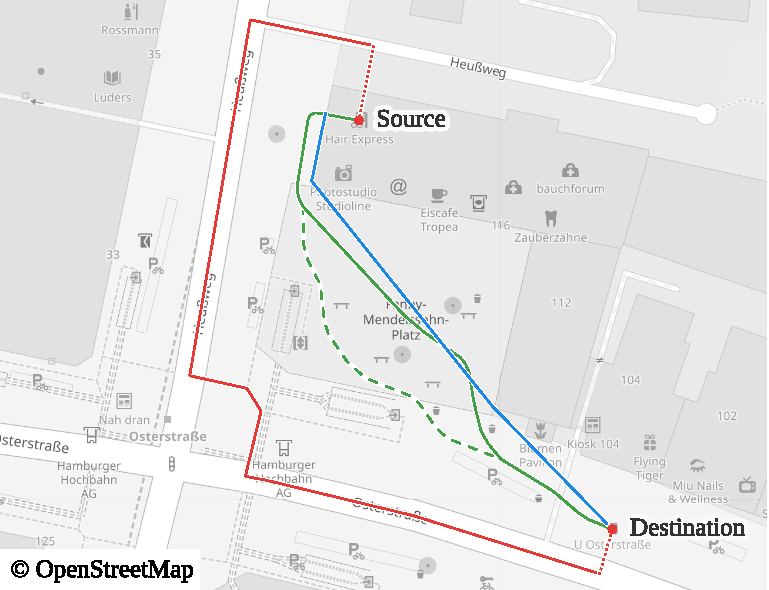
\includegraphics[width=\linewidth]{images/qgis-routing-osterstrasse}
		\end{figcenter}
		\caption[Comparison of normal routing with hybrid visibility routing.]{Comparison of an expected and realistic route (green) with a graph-based route (red) and an actual result of the algorithm presented in this work (blue).}
		\label{fig:osterstrasse-routing-vs-expected}
	\end{wrapfigure}
	
	The previous section mentions one of the disadvantages of graph-based routing:
	No assumptions can be made on whether source and destination locations are represented as vertices in the graph.
	Furthermore, trajectories of pedestrians in the real world often do not follow edges on routing graphs, which is especially the case for insufficiently connected open spaces.
	Routes strictly following the edges of a graph are therefore inaccurate for pedestrian routing\cite{graser-osm-open-spaces}, which means the calculated route contains detours and, thus, is longer than the actual trajectory and additionally may not reach the exact destination location at all.
	Such inaccuracies significantly affect the quality of agent-based simulations, as well as the helpfulness and user experience of real-world applications, such as mobile navigation apps.
	
	In this thesis, these issues are solved by proposing and designing an algorithm, called the \term{hybrid routing algorithm}, that combines the accuracy of geometric routing using visibility graphs with the optimizations and wide use of network-based routing.
	Additionally, an implementation of the proposed algorithm was created and evaluated regarding performance, correctness and usefulness.
	Determining shortest paths using the resulting approach has a simple structure, enables the use of common speedup techniques and reaches all accessible locations independent of the presence of corresponding vertices in the graph.
	Any other arbitrary location, for example, a location chosen by the user, can be added to the graph.
	Routing from and to this vertex is possible after connecting the newly added vertex to the graph.
	Real-world applications and agent-based models, which are used to simulate the behavior of pedestrians, benefit from this algorithm.

\section{Structure of this thesis}
	
	First, the basics of spatial data, data formats, graph routing, geometric routing and agent-based simulations are covered in \Cref{chap:fundamentals}.
	The scientific work related to this thesis is presented in \Cref{chap:related-work} for graphs and networks, routing techniques and pedestrian pathfinding in particular.
	In \Cref{chap:design}, the design of the system developed for this thesis is described and an overview of the different components and elements is given.
	A more detailed view of the implementation is presented in \Cref{chap:implementation}, including technical aspects of the combination of network and geometric routing as well as used frameworks.
	The hybrid routing algorithm is then evaluated in \Cref{chap:evaluation} regarding its performance, correctness and quality of the resulting routes.